% !TeX spellcheck = en_GB
% !TeX program = pdflatex
%
% LuxSleek-CV 1.1 LaTeX template
% Author: Andreï V. Kostyrka, University of Luxembourg
%
% 1.1: added tracking and letter-spacing for prettier lower caps, added `~` for language levels
% 1.0: initial release
%
% This template fills the gap in the available variety of templates
% by proposing something that is not a custom class, not using any
% hard-coded settings deeply hidden in style files, and provides
% a handful of custom command definitions that are as transparent as it gets.
% Developed at the University of Luxembourg.
%
% *NOTHING IS HARCODED, and never should be.*
%
% Target audience: applicants in the IT industry, or business in general
%
% The main strength of this template is, it explicitly showcases how
% to break the flow of text to achieve the most flexible right alignment
% of dates for multiple configurations.

\documentclass[11pt, a4paper]{article} 

\usepackage[T1]{fontenc}     % We are using pdfLaTeX,
\usepackage[utf8]{inputenc}  % hence this preparation
\usepackage[vietnamese]{babel}  
\usepackage[left = 0mm, right = 0mm, top = 0mm, bottom = 0mm]{geometry}
\usepackage[stretch = 25, shrink = 25, tracking=true, letterspace=30]{microtype}  
\usepackage{graphicx}        % To insert pictures
\usepackage{xcolor}          % To add colour to the document
\usepackage{marvosym}        % Provides icons for the contact details

\usepackage{enumitem}        % To redefine spacing in lists
\setlist{parsep = 0pt, topsep = 0pt, partopsep = 1pt, itemsep = 1pt, leftmargin = 6mm}

\usepackage{FiraSans}        % Change this to use any font, but keep it simple
\renewcommand{\familydefault}{\sfdefault}

\definecolor{cvblue}{HTML}{304263}

%%%%%%% USER COMMAND DEFINITIONS %%%%%%%%%%%%%%%%%%%%%%%%%%%
% These are the real workhorses of this template
\newcommand{\dates}[1]{\hfill\mbox{\textbf{#1}}} % Bold stuff that doesn’t got broken into lines
\newcommand{\is}{\par\vskip.5ex plus .4ex} % Item spacing
\newcommand{\smaller}[1]{{\small$\diamond$\ #1}}
\newcommand{\headleft}[1]{\vspace*{3ex}\textsc{\textbf{#1}}\par%
    \vspace*{-1.5ex}\hrulefill\par\vspace*{0.7ex}}
\newcommand{\headright}[1]{\vspace*{2.5ex}\textsc{\Large\color{cvblue}#1}\par%
     \vspace*{-2ex}{\color{cvblue}\hrulefill}\par}
%%%%%%%%%%%%%%%%%%%%%%%%%%%%%%%%%%%%%%%%%%%%%%%%%%%%%%%%%%%%

\usepackage[colorlinks = true, urlcolor = white, linkcolor = white]{hyperref}

\begin{document}

% Style definitions -- killing the unnecessary space and adding the skips explicitly
\setlength{\topskip}{0pt}
\setlength{\parindent}{0pt}
\setlength{\parskip}{0pt}
\setlength{\fboxsep}{0pt}
\pagestyle{empty}
\raggedbottom

\begin{minipage}[t]{0.33\textwidth} %% Left column -- outer definition
%  Left column -- top dark rectangle
\colorbox{cvblue}{\begin{minipage}[t][5mm][t]{\textwidth}\null\hfill\null\end{minipage}}

\vspace{-.2ex} % Eliminates the small gap
\colorbox{cvblue!90}{\color{white}  %% LEFT BOX
\kern0.09\textwidth\relax% Left margin provided explicitly
\begin{minipage}[t][293mm][t]{0.82\textwidth}
\raggedright
\vspace*{2.5ex}

\Large Trần \textbf{\textsc{Tấn Phát}} \normalsize 

% Centering without extra vertical spacing
\null\hfill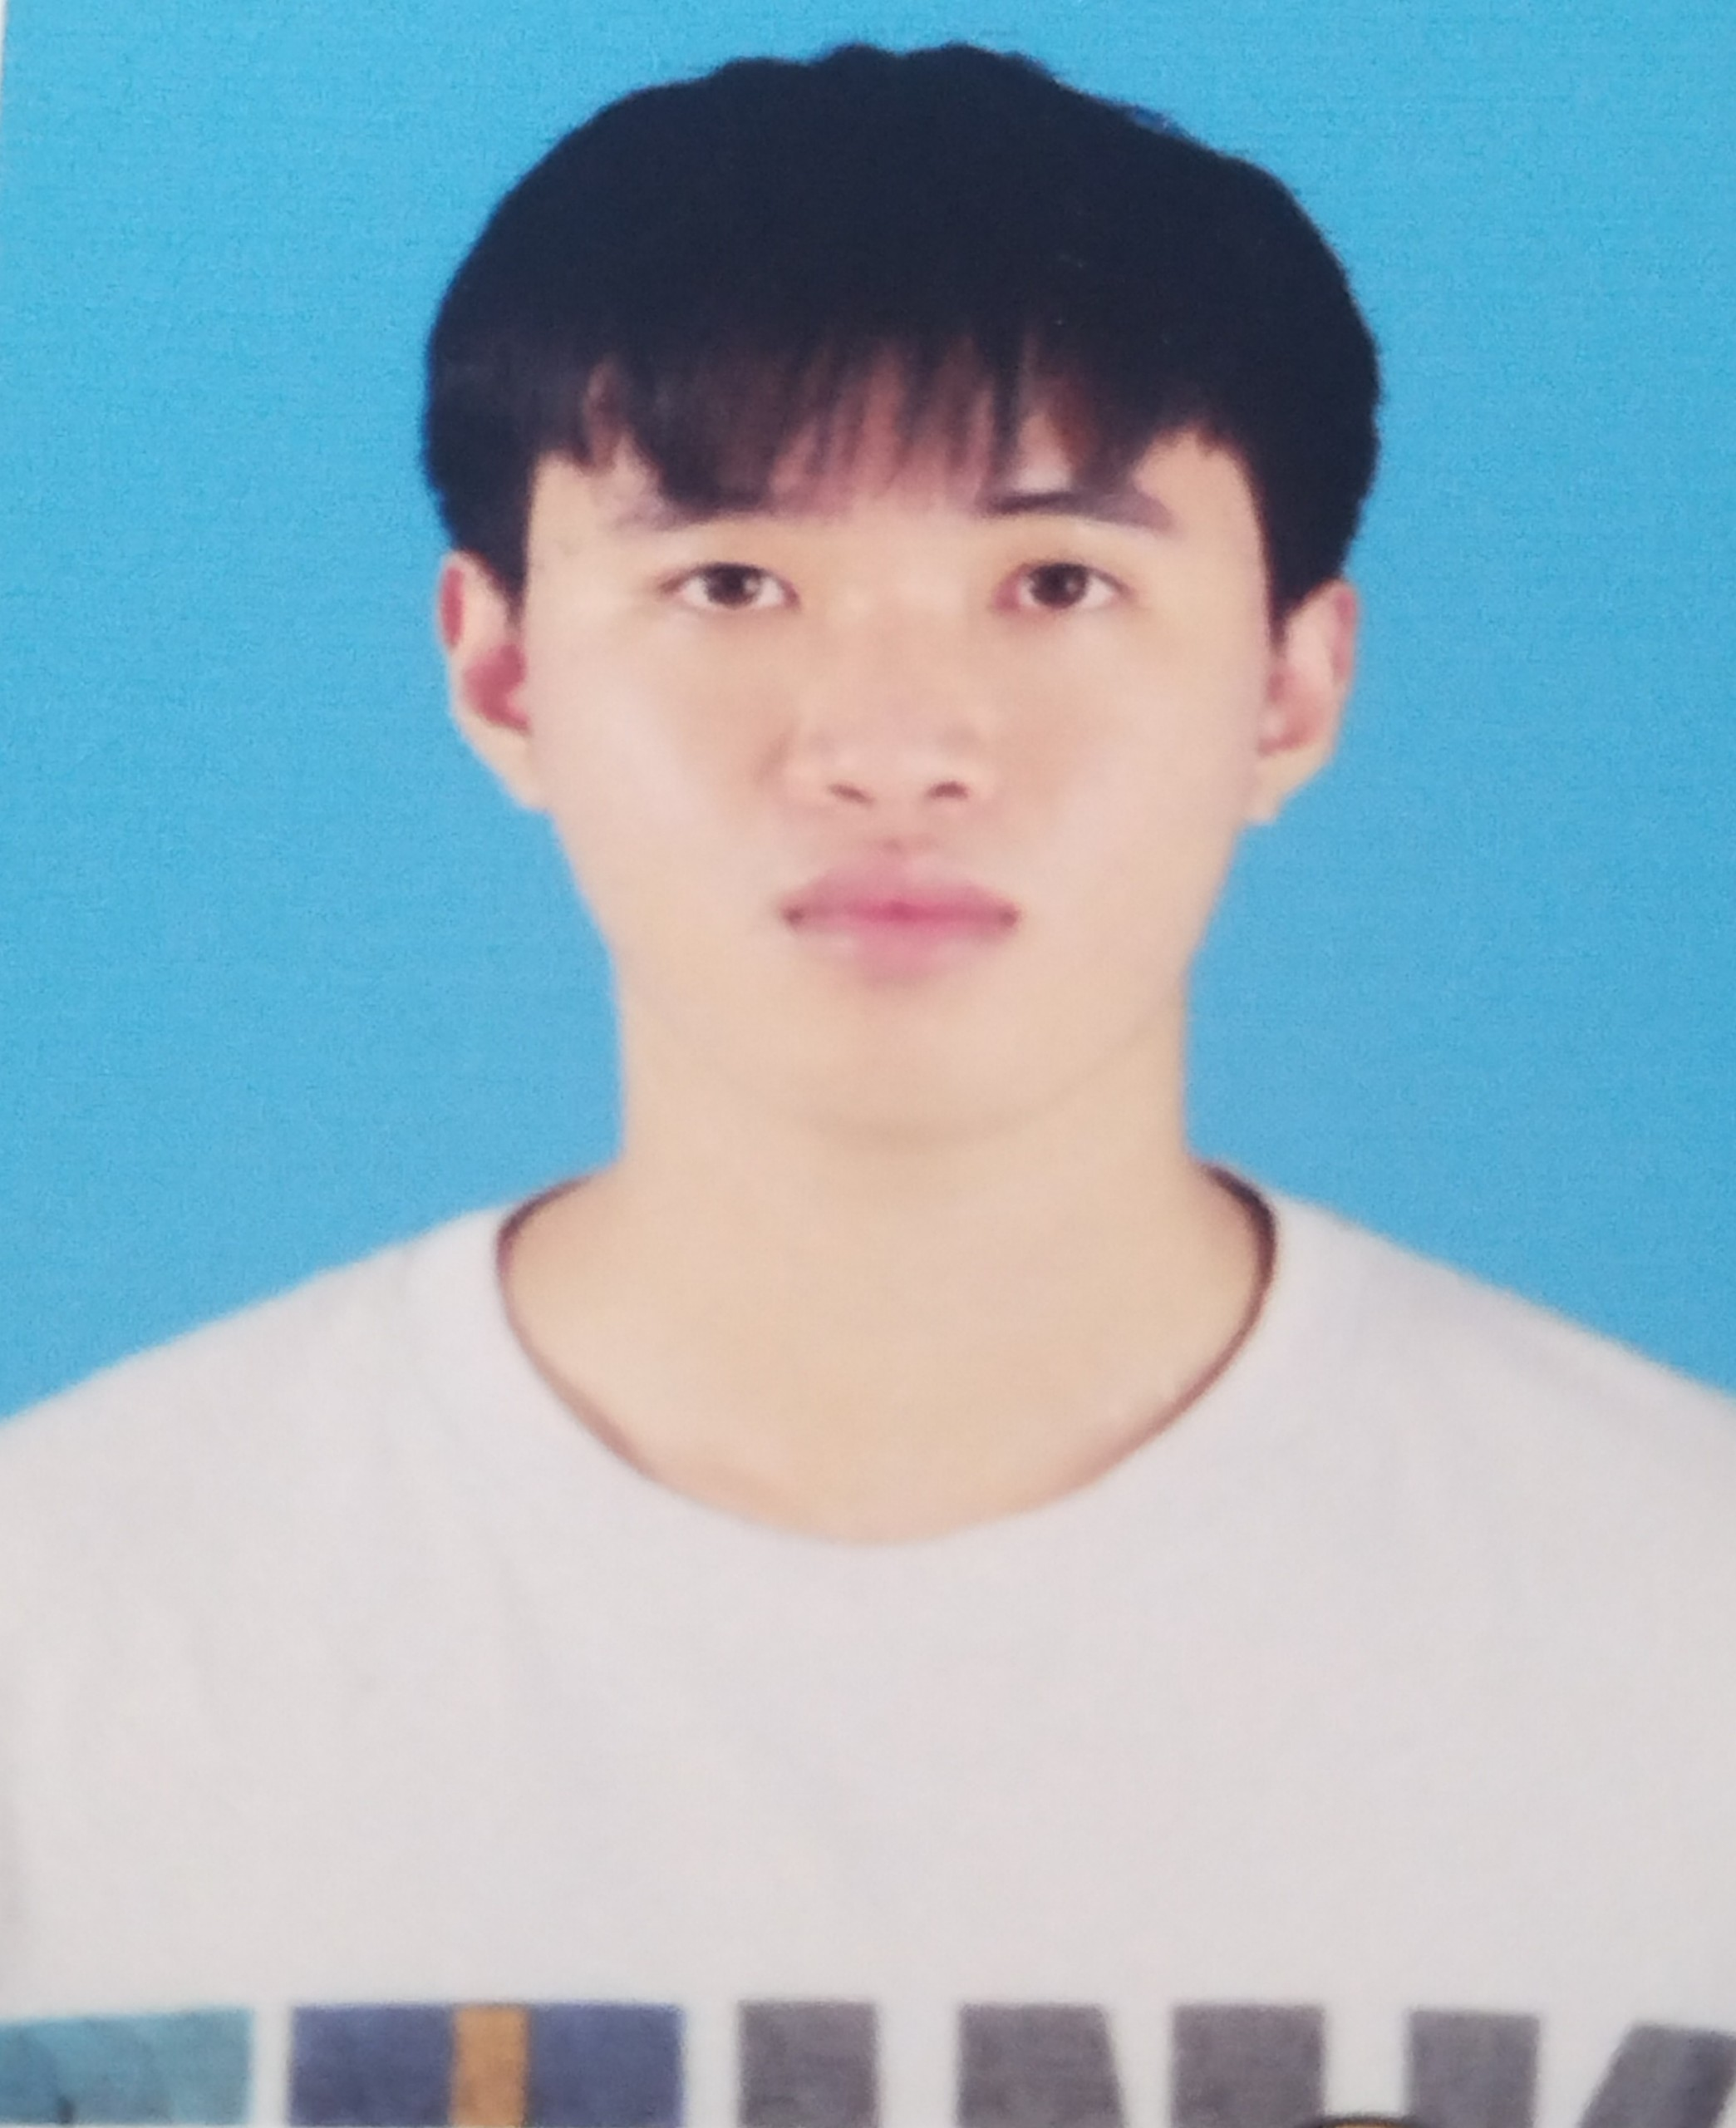
\includegraphics[width=0.65\textwidth]{Trần Tấn Phát.jpg}\hfill\null

\vspace*{0.5ex} % Extra space after the picture
\begin{figure}
    \centering
    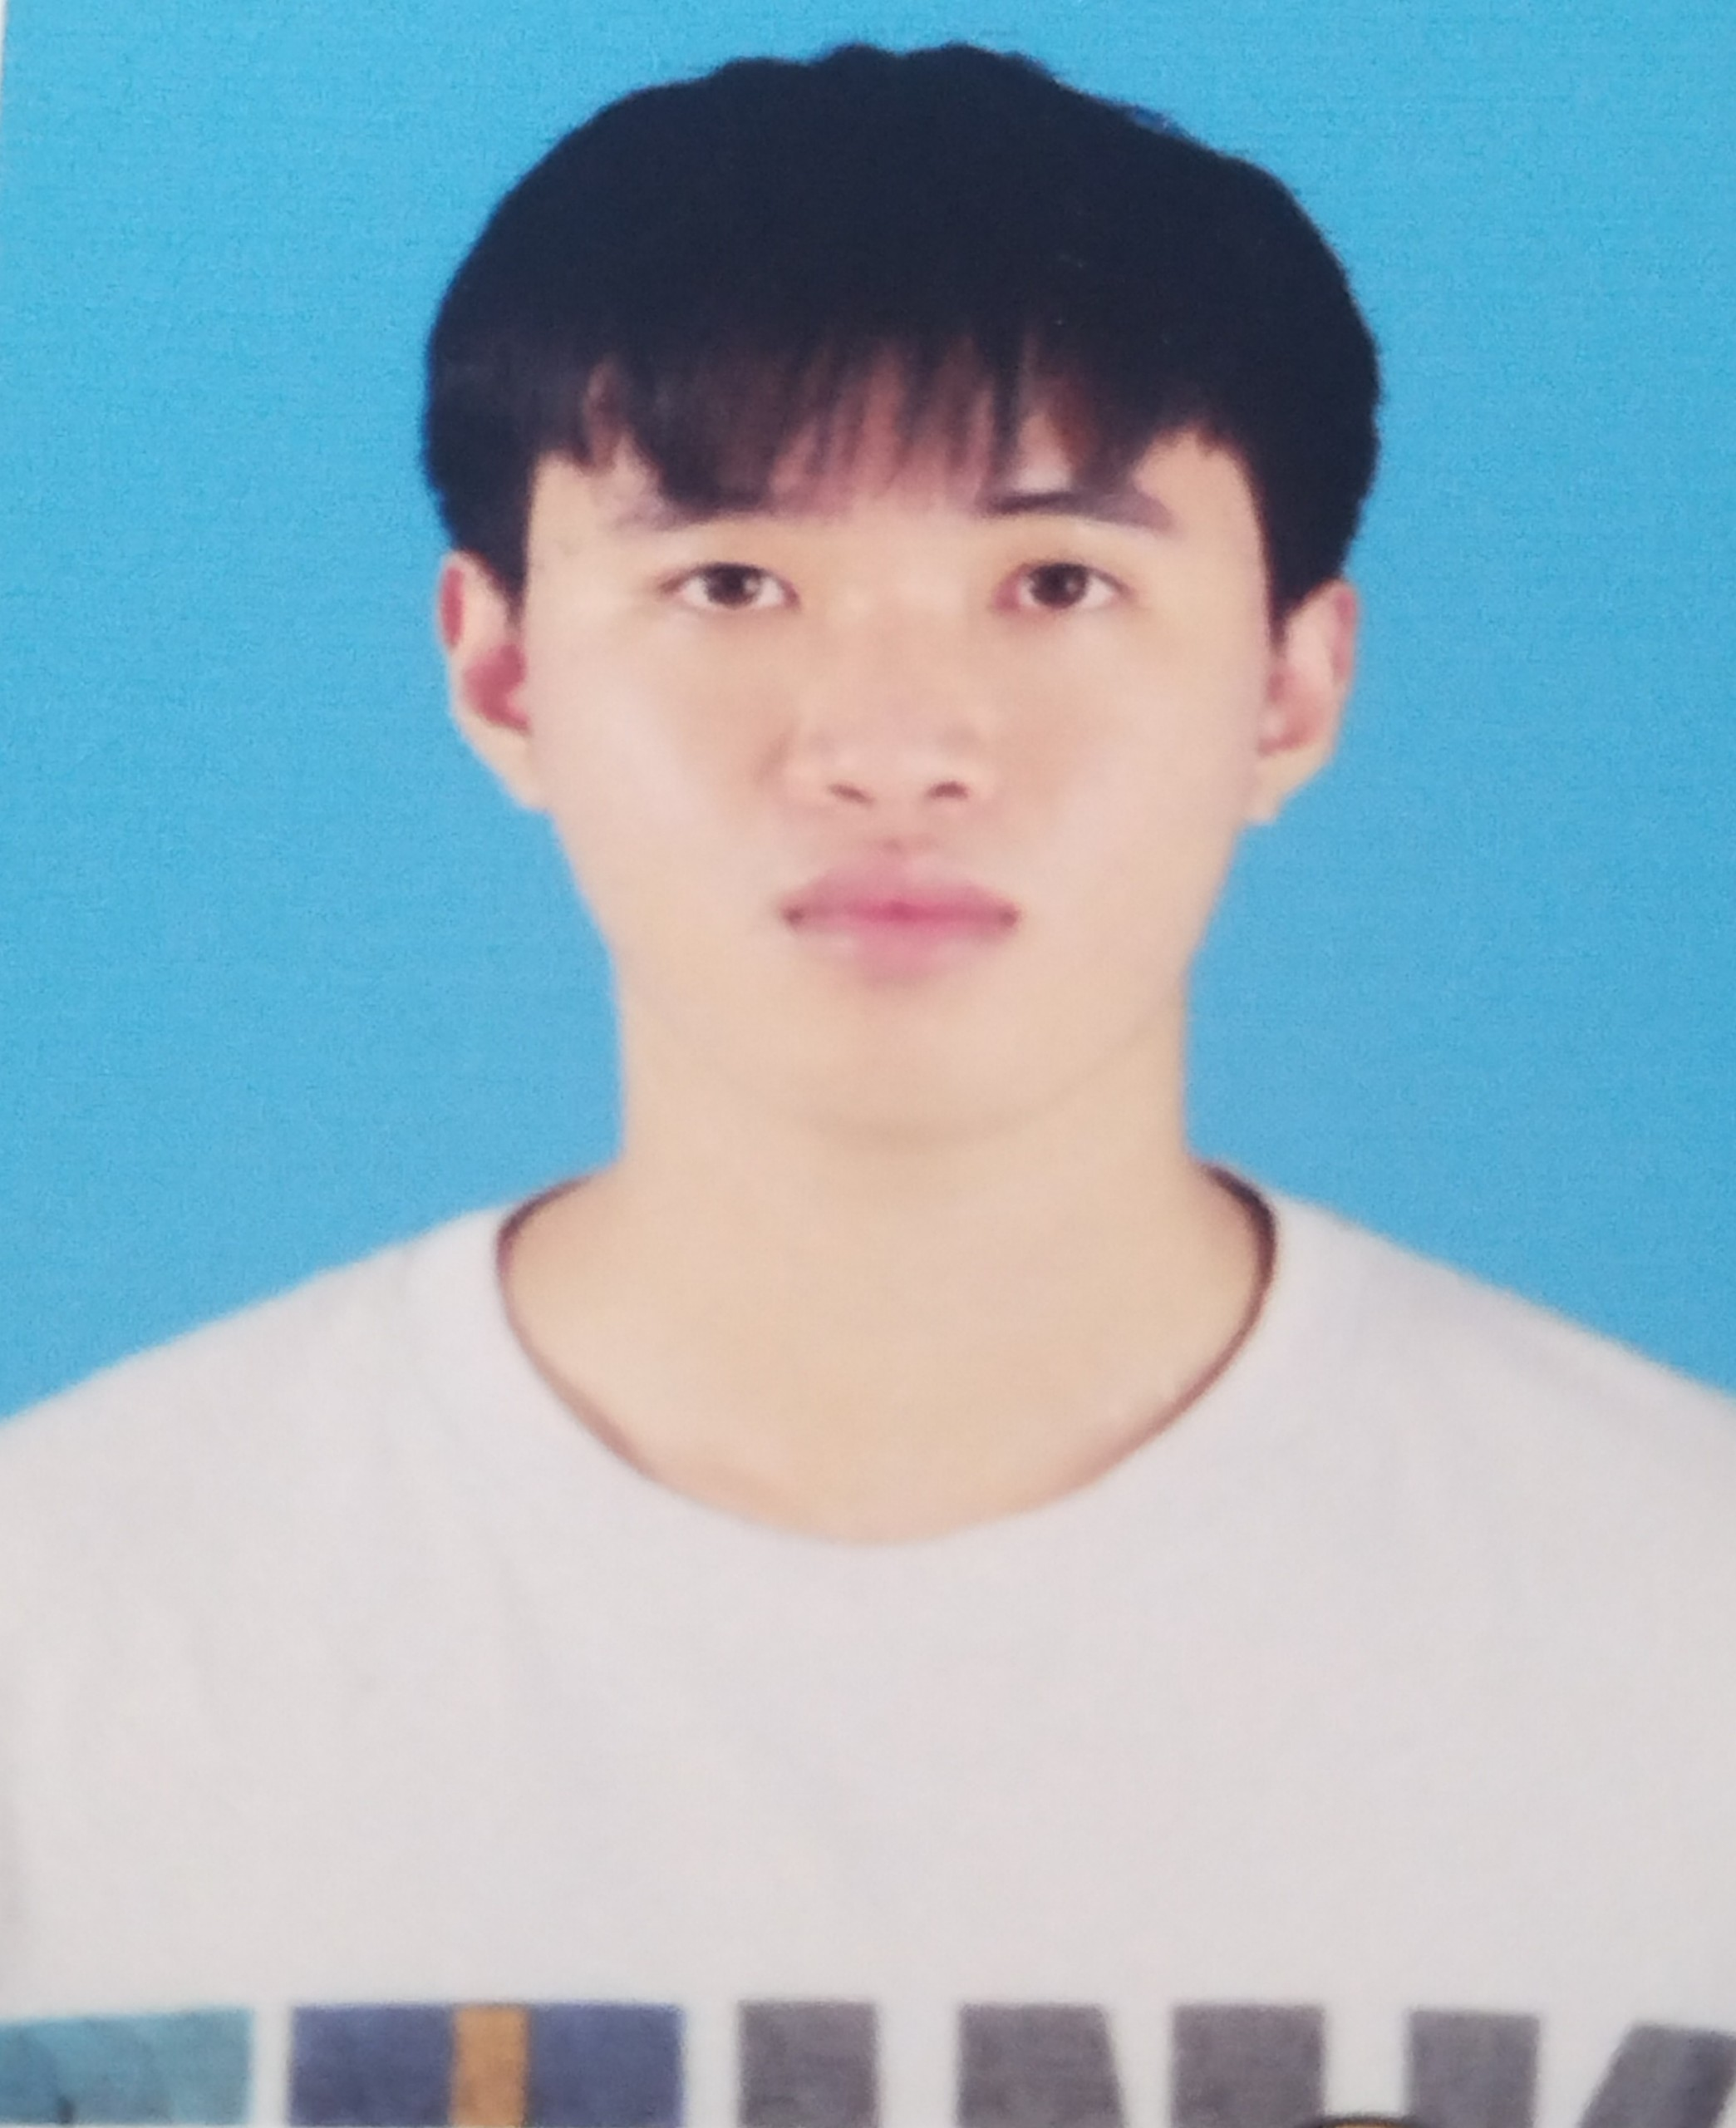
\includegraphics[width=0.5\linewidth]{Trần Tấn Phát.jpg}
    \caption{Enter Caption}
    \label{fig:enter-label}
\end{figure}
\headleft{Lý lịch}
\textit{Kỹ sư phần mềm} với hơn 6 năm kinh nghiệm trong JavaScript, HTML,Python,SQL,C++,..Thông thạo các kỹ năng mã hóa, kiểm tra phiên bản,... . Có kiến thức sâu rộng về dữ liệu và giải thuật, khung phần mềm, hệ điều hành, cơ sở dữ liệu,... Đã từng tham gia nhiều dự án phần mềm với số lượng người dùng lớn.

\headleft{Contact details}
\small % To fit more content
\MVAt\ {\small trantanphat.stu@gmail.com} \\[0.4ex]
\Mobilefone\ 0348183773 \\[0.5ex]
\Letter\ 128A Tân Lập,Bình Thắng, Dĩ An, Bình Dương
\normalsize

\headleft{Thông tin cá nhân}
\textbf{Ngày sinh: 29/05/2006} \\[0.5ex]
Quốc tịch: \textbf{Việt Nam} \\[0.5ex]
Ngôn ngữ giao tiếp: \textbf{Tiếng Việt}, \textbf{Tiếng Anh}, \textbf{Tiếng Nhật}, \textbf{Tiếng Hàn Quốc}, \textbf{Tiếng Tây Ban Nha}, \textbf{Tiếng Đức}

\headleft{Thông thạo}
\begin{itemize}
\item SQL, SSMS, Power BI,Power BI Service, DAX Functions,
Tableau, Python, PySpark
\item Panda, Numpy, Warehouse, Azure Databricks
\item Microsoft Excel, MS Word,MS PowerPoint
\item SQL Server, T-SQL, Kibana,Eclipse Birt,ETL
\item JavaScript, HTML, GitHub
\item Kỹ năng giao tiếp và làm việc nhóm
\end{itemize} 

\end{minipage}%
\kern0.09\textwidth\relax%%Right margin provided explicitly to stretch the colourbox
}
\end{minipage}% Right column
\hskip2.5em% Left margin for the white area
\begin{minipage}[t]{0.56\textwidth}
\setlength{\parskip}{0.8ex}% Adds spaces between paragraphs; use \\ to add new lines without this space. Shrink this amount to fit more data vertically

\vspace{2ex}

\headright{Kinh nghiệm}

\textsc{Kỹ sư phần mềm} tại \textit{Fujinet (Hồ Chí Minh).}  \dates{08/2030--05/2036} \\

\smaller{Có kinh nghiệm làm việc trong nhiều dự án phát triển phần mềm cả trong nước và ngoài nước.}

\is
\smaller{Leading engineer của nhóm 8 người phát triển ứng dụng Fnat với hơn 1 triệu người dùng.}

\is
\smaller{Tham vấn kỹ thuật cho dự án BNA Smart Home đã được ứng dụng trong hơn 100000 căn hộ, chung cư, nhà ở,...cả trong nước và ngoài nước.}

\is
\smaller{Đồng sáng tác cuốn "Dữ liệu, giải thuật và kẻ khù khờ". Sách về lập trình bán chạy nhất Đông Nam Á 2025 }

\is
\smaller{Thành viên của đội HCMUS Coding Phoenix, vô địch cuộc thi ICPC Châu Á 2027  }

\is 
\smaller{Có nhiều kinh nghiệm phát triển phần mềm trong các dự án freelance}

\is
\smaller{Thông thạo nhiều ngôn ngữ lập trình như Javascript, Java, Python, SQL, C++, C.} 


\is
\smaller{Hiểu biết sâu rộng về cấu trúc dữ liệu, các quy trình phát triển phần mềm.}

\headright{Education}

\textsc{Thạc Sĩ Khoa Học Máy Tính.} \textit{Trường Đại Học Khoa học Tự Nhiên, Đại Học Quốc Gia Thành Phố Hồ Chí Minh}. \dates{2028--2031} \\

\is
\textsc{Cử nhân khoa công nghệ thông tin.} \textit{Trường Đại Học Khoa học Tự Nhiên, Đại Học Quốc Gia Thành Phố Hồ Chí Minh}.  \dates{2024--2028} \\

\headright{Chứng chỉ}

\smaller{\textsc{CS50, Đại Học Harvard,}} 
\is
\smaller{\textsc{AWS Certified Solutions Architec, Amazon Web Service.}} \dates{July-3-2024} \\
\is
\smaller{\textsc{SQL, Hacker Rank}}

\headright{Sở thích}

\textit{Đọc sách,cầu lông, tham gia các hoạt dộng tình nguyện,... }\\
\begin{figure}
    \centering
    \includegraphics[width=0.5\linewidth]{lê sâng húc.jpg}
    \caption{Enter Caption}
    \label{fig:enter-label}
\end{figure}
\textit{Nâng cao kỹ năng lập trình, tham gia các diễn đàn công nghệ thông tin}
\end{minipage}

\end{document}
